\documentclass{article}
\usepackage{booktabs}
\usepackage{graphicx}
\usepackage{amsmath}
\usepackage[a4paper, total={7in, 10.5in}]{geometry}
\usepackage[toc,page]{appendix}
\usepackage{listings} % Listing package to add appendix
\usepackage{xcolor}   % Custom colors
\usepackage{graphicx}  % Required to include images
\usepackage{hyperref}% to put links
\usepackage{float} %to place correctly pictures
\usepackage{cite} %for better citations

\hypersetup{
    colorlinks=true,
    linkcolor=blue,
    urlcolor=blue,
    citecolor=red,
    linktoc=all,    % Links entire section titles in the ToC
    linkcolor=black % Sets ToC links to black; other links remain as specified
}

% Defining colors for the python section
\definecolor{codegreen}{rgb}{0,0.6,0}
\definecolor{codeblue}{rgb}{0,0,0.8}
\definecolor{codepurple}{rgb}{0.58,0,0.82}
\definecolor{codebackground}{rgb}{0.95,0.95,0.92}
\begin{document}

\title{Mid term Exam for Financial Econometrics with Python}
\author{PRAT Paul; GAVINI Charles; FOURNIER Justin; BLANC Mathieu}
\date{\today}

\maketitle %showcase the title in the top of the page with the informations upper

\tableofcontents %creating a table of contens

%first, introduction
\section{Introduction}


This document provides a comprehensive presentation of our results, 
including all relevant tables, figures, and calculations. 
The report is structured into distinct parts, beginning with the importation of essential Python libraries. 
We then initialize variables to organize the data into different categories (e.g., daily, monthly, returns, log returns), 
allowing for clear analysis and comparison across various data types and intervals.


\section{Preliminary}
%Instructions


%At the beginning of your answer to Question 1, indicate clearly:
%- the name and the exact ticker of stock or index you are considering,
%- the length of your sample (number of days, months, years),
%- the initial and final dates of your sample, and
%- the stock market and country in which the stock you selected is traded, or to which the stock index you selected refers to.
%Using the time series you downloaded in PRELIMINARY STEP 1, compute the log-returns at daily, 
%monthly, and annual frequencies and present a table of summary statistics of these three series of returns. 
%The table should be similar to the one appearing in slide n. 91 of the set of slides titled 
%``Lecture 1: Financial Returns: Description and Stylized Facts’’.
\subsection{AMAZON}

The selected stock for this analysis is Amazon due to its significant relevance in current global markets, its impressive growth over time and its position as a major industry leader.
The ticker from yahoo finance is "\textbf{\textit{AMZN}} " on the Nasdaq stock exchange \href{https://finance.yahoo.com/quote/AMZN/.}{AMAZON on Yahoo Finance}
First, importing the Amazon stock with yfinance, then display the pandas table.
We will import 25 years, 8 months and 25 days of data (from 1999-01-21 to 2024-10-16).

\subsection{Data Table}
The data printed here is the preview of the Amazon stock extraction from yahoo finance:
% LaTeX table from 'table.tex'
\begin{table}[h!]
    \centering
    \begin{tabular}{lrrrrrr}
\toprule
{} &      Open &      High &       Low &     Close &  Adj Close &     Volume \\
Date       &           &           &           &           &            &            \\
\midrule
1999-09-16 &  0.051563 &  0.052083 &  0.050260 &  0.050911 &   0.046693 &  158112000 \\
1999-09-17 &  0.050586 &  0.051042 &  0.048958 &  0.050781 &   0.046574 &  171648000 \\
1999-09-20 &  0.049870 &  0.050521 &  0.048958 &  0.048958 &   0.044902 &  229104000 \\
1999-09-21 &  0.047917 &  0.048177 &  0.043620 &  0.044271 &   0.040603 &  737328000 \\
1999-09-22 &  0.044271 &  0.045573 &  0.041667 &  0.045313 &   0.041559 &  375984000 \\
\bottomrule
\end{tabular}
  
    \caption{Preview of Amazon Stock Data from Yahoo Finance}
    \label{tab:amazon_stock_preview}
\end{table}



\subsection{Checking the 25 Years range condition}


We need to verify that the data displays accurately over the 25 years range. 
Fortunately, the extracted  Amazon data has been available since January 1999. 
To ensure the data’s continuity and completeness, we will implement a Python script that identifies and counts any gaps within the dataset. 
By visualizing the dates of these gaps, we can easily detect any significant interruptions that could potentially impact our data analysis

\begin{figure}[H]
    \centering
    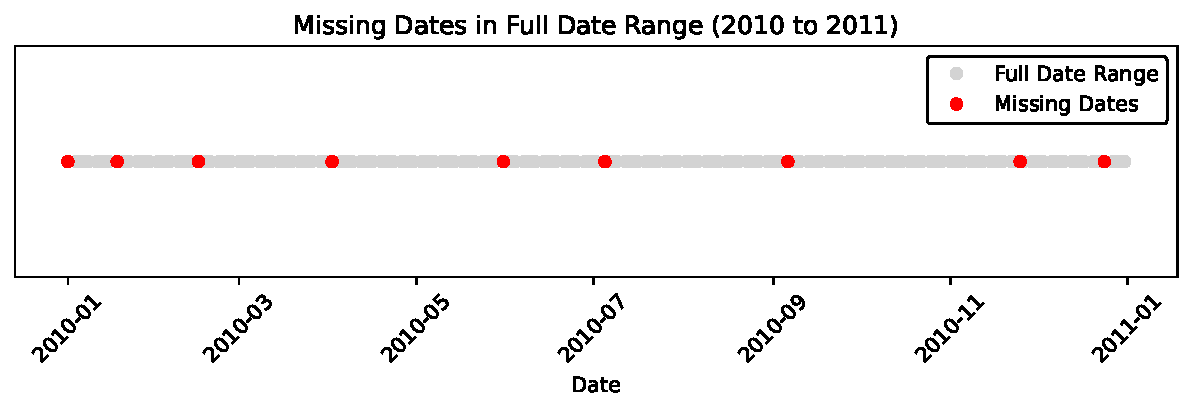
\includegraphics[width=0.8\textwidth]{Img/MissingDates(2010_to_2011).pdf}
    \caption{Missing Dates in Full Date Range (2010 to 2011)}
    \label{fig:missing_dates}
\end{figure}

\noindent We identified a total of 238 isolated days of data gaps per year across the 25-years range (6476 values). 
Therefore, the data remains reliable for our stylized facts analysis. 
The missing data points in our dataset are randomly distributed and account for 3.7\% of the total data. 
According to scientific studies on data reliability for volatility testing, a dataset with up to 10% missing data is considered reliable for statistical testing.
\cite{pumi2023longrange} 

\section{First Results}

\subsection{Prices Evolutions}

With the accuracy and the reliability of our dataset confirmed, we begin by plotting the evolution of prices over 4 different periods : Daily, Weekly, Monthly and Yearly prices.

\begin{figure}[H]
    \centering
    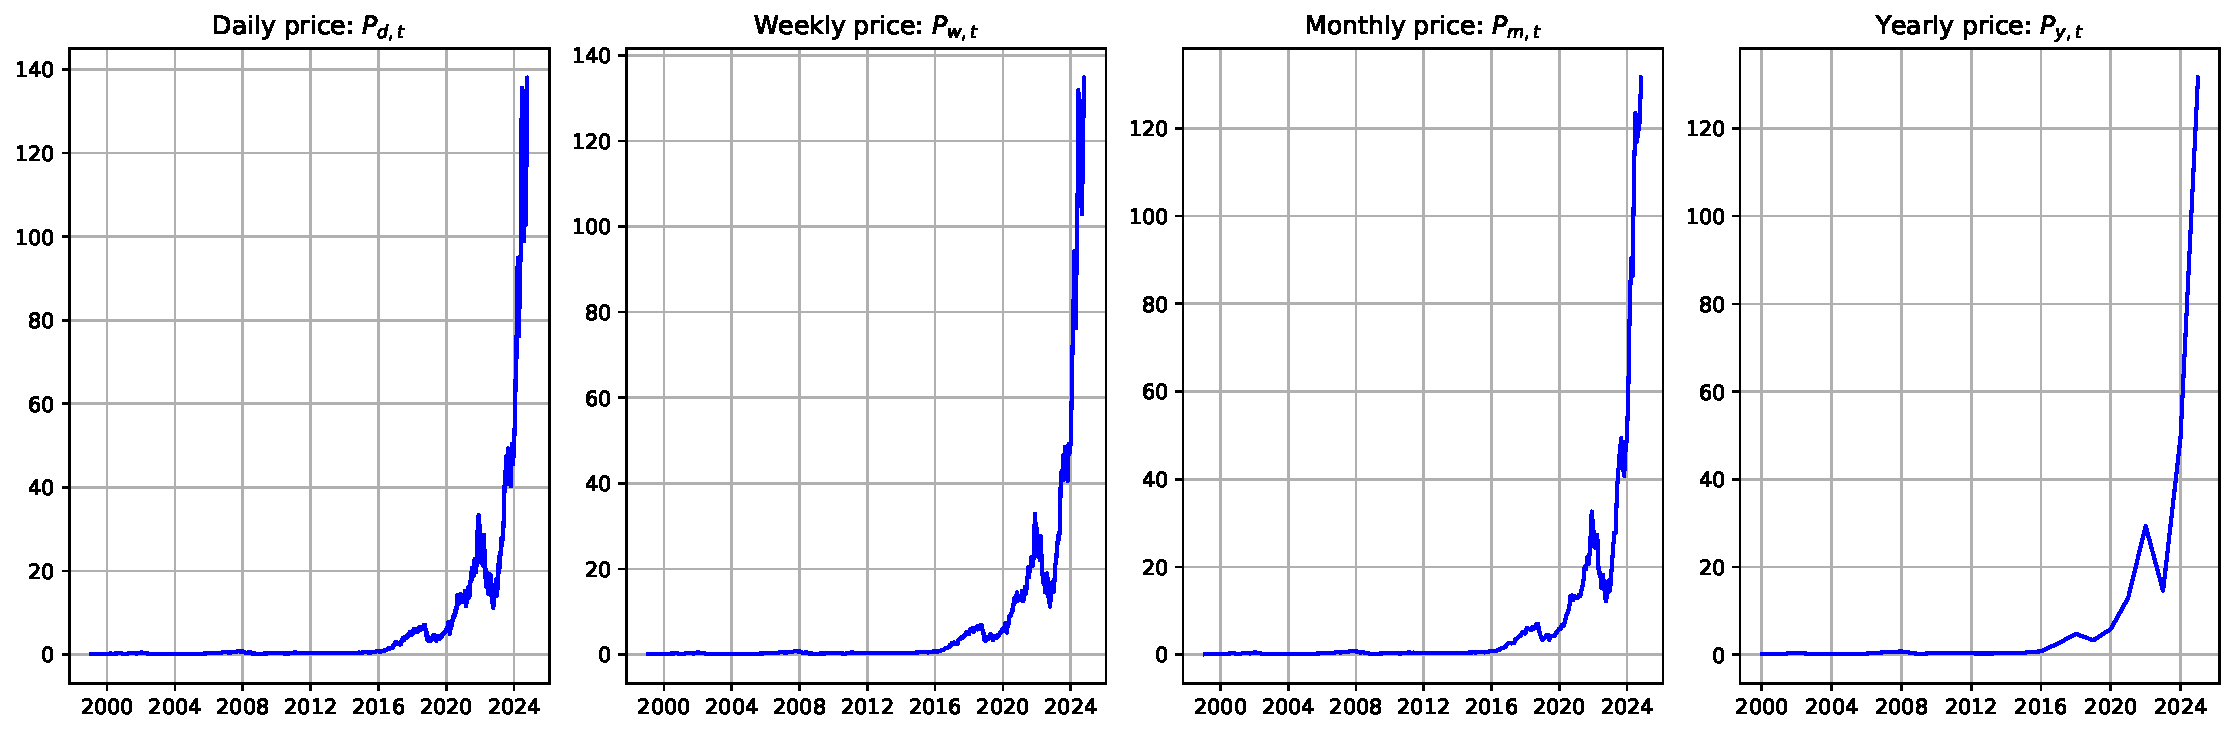
\includegraphics[width=\textwidth]{Img/prices_time.pdf}
    \caption{Prices over time by frequency}
    \label{fig:prices_time}
\end{figure}

\subsection{Calculating Returns}
Using the processed data, we can now output graphs for several key metrics: 
daily prices, daily log prices, daily simple returns, and daily log returns. 
Plotting these metrics will allow us to observe daily price movements, 
the transformation of prices into $log$ form for trend analysis, 
as well as daily returns and their logarithmic equivalents.
\begin{figure}[H]
    \centering
    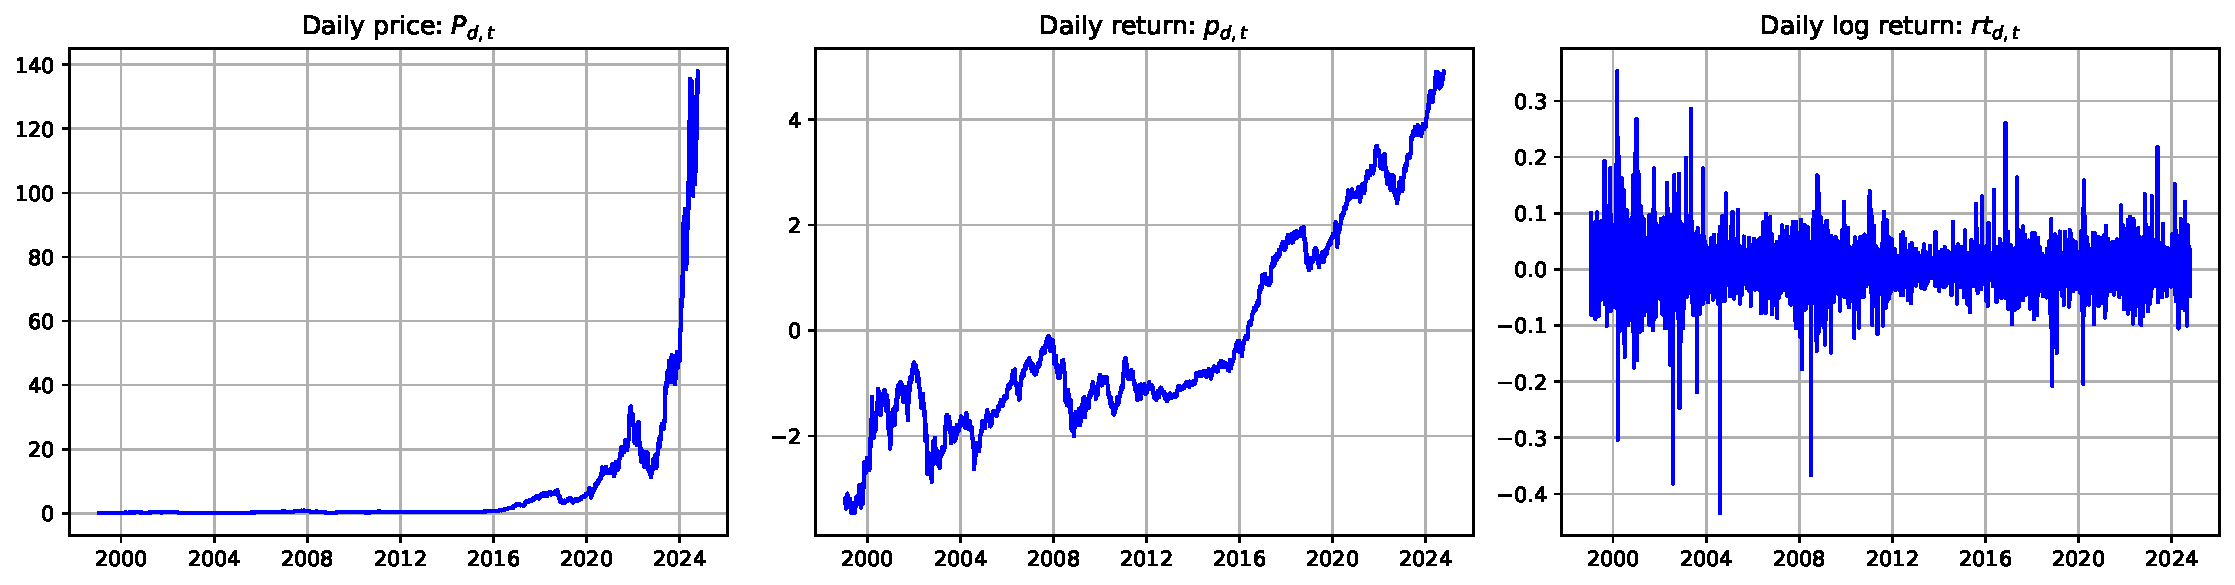
\includegraphics[width=\textwidth]{Img/log_returns.pdf}
    \caption{Prices, returns and log returns}
    \label{fig:log_returns}
\end{figure}

\subsection{Squared Returns}

To complete the analysis of daily price data, we also plot the daily squared returns and daily squared log returns, 
(providing us a key insight on the volatile behavior on the potential stock risk of our data set.)
\begin{figure}[H]
    \centering
    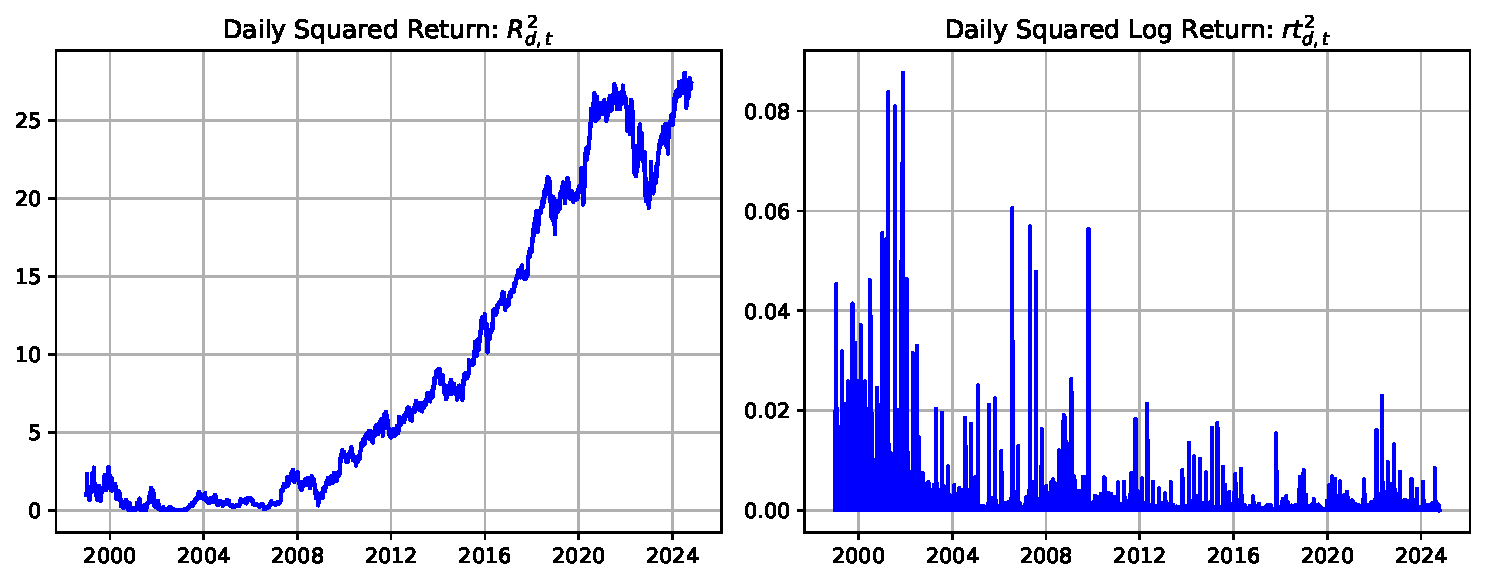
\includegraphics[width=0.8\textwidth]{Img/squared_log_returns.pdf}
    \caption{Squared daily returns and daily log returns}
    \label{fig:squared_logreturns}
\end{figure}

\section{Amazon and the 8 Stylized Facts}

\subsubsection{Summary statistics}


\begin{table}[H]
    \centering
    \begin{tabular}{lrrrr}
\toprule
{} &        daily &      weekly &    monthly &     annual \\
\midrule
Mean                    &      0.06351 &     0.31014 &    1.32164 &   22.85692 \\
St.Deviation            &      3.24131 &     6.76830 &   13.06275 &   45.28052 \\
Diameter.C.I.Mean       &      0.07896 &     0.36213 &    1.45887 &   18.11598 \\
Skewness                &      0.41992 &     0.05008 &   -0.45895 &   -0.15137 \\
Kurtosis                &     11.15158 &     7.60655 &    2.59462 &   -0.64793 \\
Excess.Kurtosis         &      8.15158 &     4.60655 &   -0.40538 &   -3.64793 \\
Min                     &    -28.45678 &   -38.51804 &  -53.02674 &  -68.54809 \\
Quant5                  &     -4.61051 &    -9.74288 &  -20.16713 &  -55.72274 \\
Quant25                 &     -1.25994 &    -2.64062 &   -4.98163 &   -7.23999 \\
Median                  &      0.04108 &     0.30519 &    2.09626 &   23.07665 \\
Quant75                 &      1.39659 &     3.40897 &    8.45973 &   55.96192 \\
Quant95                 &      4.47118 &    10.67416 &   20.90661 &   94.77653 \\
Max                     &     29.61811 &    56.11507 &   48.35221 &  102.44636 \\
Jarque.Bera.stat        &  33735.75720 &  3235.87866 &   97.20696 &    0.51147 \\
Jarque.Bera.pvalue.X100 &      0.00000 &     0.00000 &    0.00000 &   77.43487 \\
Lillie.test.stat        &      0.10194 &     0.09591 &    0.08194 &    0.06494 \\
Lillie.test.pvalue.X100 &      0.10000 &     0.10000 &    0.10000 &   99.00000 \\
N.obs                   &   6474.00000 &  1342.00000 &  308.00000 &   24.00000 \\
\bottomrule
\end{tabular}
  
    \caption{Summary statistics for the amazon stock}
    \label{tab:Stylized_facts_preview}
\end{table}


% refering to the table with : Table~\ref{tab:Stylized_facts_preview}

\subsection{Prices are non-stationary}

The first feature that will highlight non-stationarity of
the prices is the comparison of \( p_t \) vs \( p_{t-1} \).

\begin{figure}[H]
    \centering
    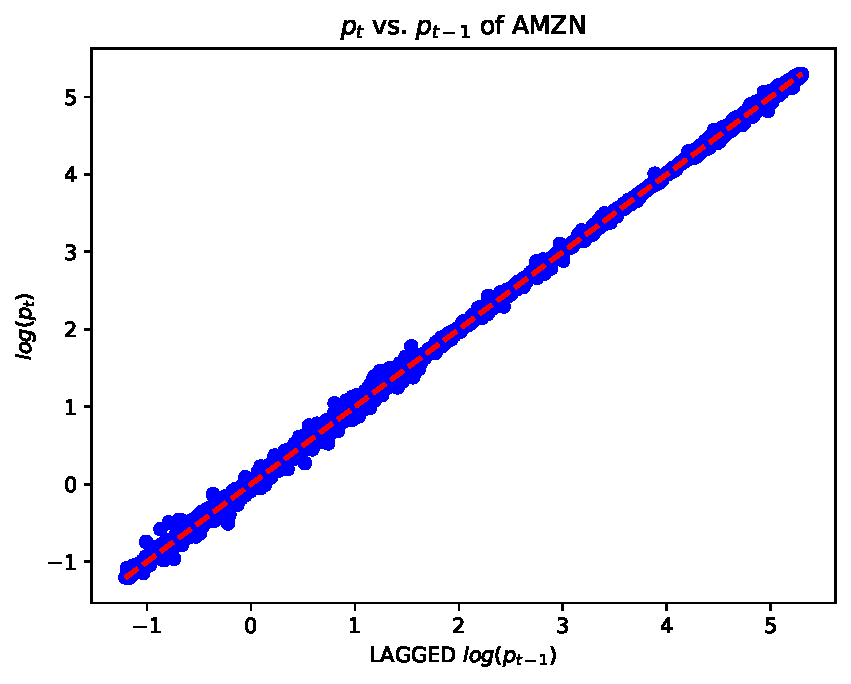
\includegraphics[width=0.5\textwidth]{Img/Laggedlog(p_t-1).pdf}
    \caption{Comparison of \( \log(p_t) \) vs \( \log(p_{t-1}) \)}
    \label{fig:LogptVSLogpt-1}
\end{figure}

\noindent The graph in Figure \ref{fig:LogptVSLogpt-1} demonstrates this strong linear 
relationship, indicating that Amazon's prices at time \( t \) are highly dependent on those at \( t-1 \) and lack mean reversion,
 supporting the idea of non-stationarity.

\noindent Additionally, the empirical autocorrelation function (ACF) of Amazon's daily prices shows a slow decay, further suggesting non-stationarity, as shown in the next figure.

\begin{figure}[H]
    \centering
    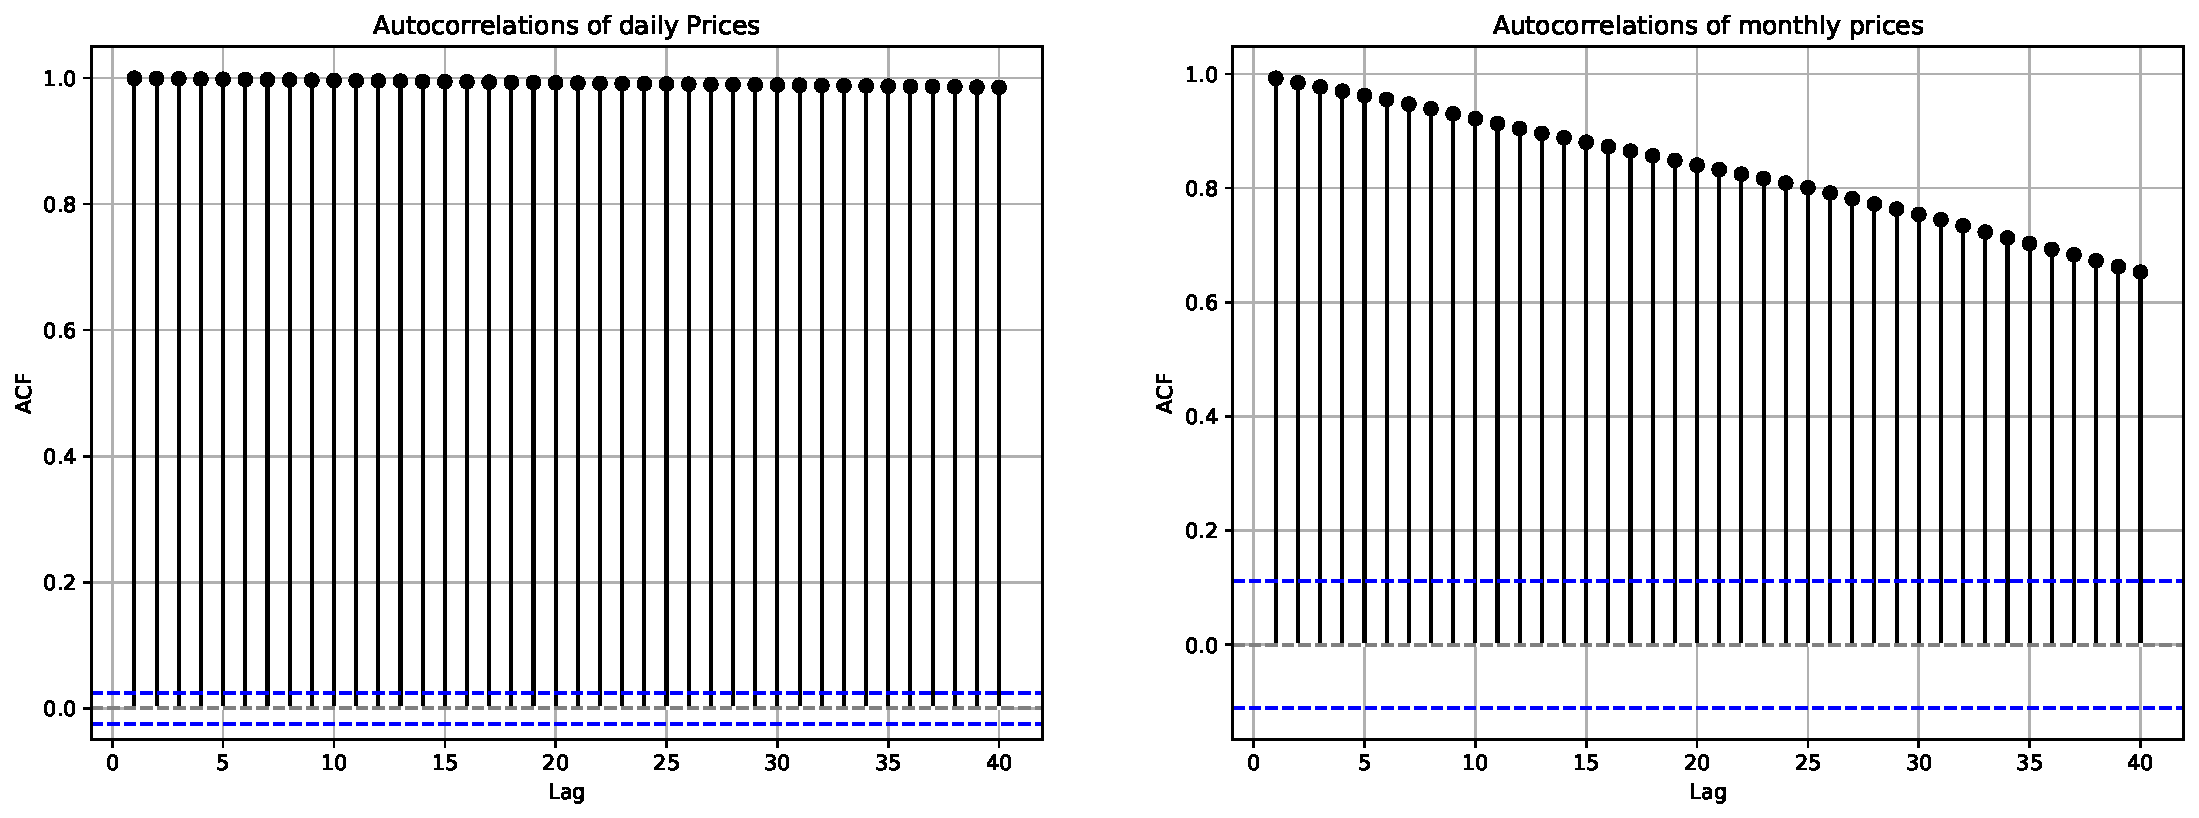
\includegraphics[width=0.8\textwidth]{Img/Autocorrel_daily_monthly.pdf}
    \caption{Autocorrelations of daily and monthly Prices (1999-2024)}
    \label{fig:Autocorrelations_daily_monthly}
\end{figure}

\subsection{Returns are stationary}
TODO
\subsection{Asymmetry}
TODO
\textbf{Stylized Fact 3: The distribution of returns is asymmetric and often negatively skewed}, reflecting the fact that the downturns of financial markets are often much steeper than the recoveries. Investors tend to react more strongly to negative news than to positive news.

\begin{figure}[H]
    \centering
    \begin{minipage}{0.45\textwidth}
        \begin{table}[H]
            \centering
            \begin{tabular}{lrrrr}
\toprule
{} &     daily &   weekly &  monthly &   annual \\
\midrule
Skewness &   0.39404 &  0.04813 & -0.46401 & -0.99033 \\
Kurtosis &  11.04424 &  7.51963 &  2.60379 &  1.46124 \\
\bottomrule
\end{tabular}
  
            \caption{Skewness and kurtosis for $log$ returns}
            \label{tab:skewness_kurtosis}
        \end{table}
    \end{minipage}
    \hspace{0.05\textwidth}
    \begin{minipage}{0.45\textwidth}
        \centering
        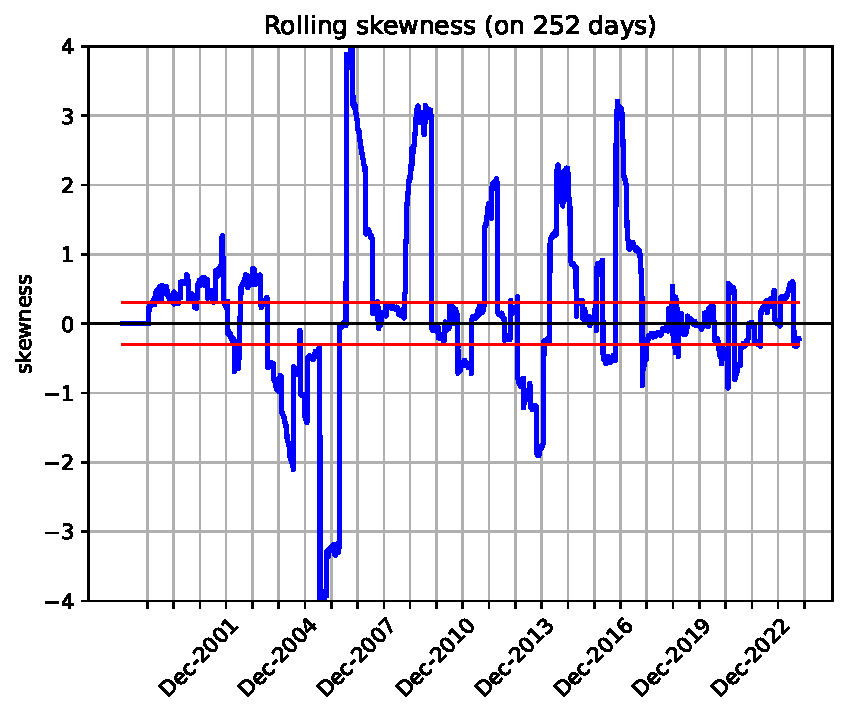
\includegraphics[width=0.8\textwidth]{Img/Fact3_2_rollskew.pdf}
        \caption{Rolling skewness}
        \label{fig:Rolling_skewness}
    \end{minipage}
\end{figure}


\subsection{Heavy tails}
TODO
\subsection{Gaussianity}
TODO
\subsubsection{High frequency non-Gaussianity}

\noindent As the result in Table~\ref{tab:Stylized_facts_preview} 
the skewness is positive for daily and monthly data \cite{Skewness} TODO add an article about amzn skewness.
The 3\textsuperscript{rd} central moment is defined as
$\mu_3 := E((X - m_1)^3).$ The skewness of \( r_t \) is defined as:
\[
\text{Skew}(r_t) := E \left[ \left( \frac{X - m_1}{\sigma} \right)^3 \right] = \frac{\mu_3}{\sigma^3} = \frac{\mu_3}{\mu_2^{3/2}}.
\]
In this case, and as emphasized in the $3^{rd}$ stylized fact, \( \text{Skew}(r_t) >0 \), large realizations of \( X \) are more often larger
than the mean \( \mu \). 
Skewness is thus used as a measure of asymmetry of the distribution \( f_X(x) \). Therefore:
 
\( \text{Skew}(r_t) > 0 \), so the distribution is said to be \textbf{right skewed}. 
%For symmetric distributions (e.g., Gaussian, t-Student, uniform), 
%we have \( \text{Skew} = 0 \). In these cases, all odd moments are zero:
%\( \mu_r = E[(X - \mu)^3] = 0 \) for \( r = 3, 5, \dots \)

\( \text{Skew}(r_t) > 0 \), then \( \mu > \text{median} \), where the median is the 50\% quantile of the distribution.

\subsubsection{Aggregational Gaussianity}
TODO
\subsection{Returns are not autocorrelated}
TODO
\subsection{Volatility clustering and long range dependence of squared returns}
TODO
\subsection{Leverage effect}
TODO

\appendix

\lstset{
    language=Python,
    backgroundcolor=\color{codebackground},   % Background color
    basicstyle=\ttfamily\footnotesize,        % Font and size
    breaklines=true,                          % Automatic line breaking
    frame=single,                             % Frame around code
    numbers=left,                             % Line numbers on the left
    numberstyle=\tiny\color{gray},            % Line number style
    keywordstyle=\color{codeblue}\bfseries,   % Keyword color
    commentstyle=\color{codegreen}\itshape,   % Comment color
    stringstyle=\color{codepurple},           % String color
    showstringspaces=false,                   % Hide string spaces
    captionpos=b,                             % Caption position: bottom
    tabsize=4                                 % Tab width
}

\section{Appendix: Python Code}
Below is the Python code used in the analysis.

\begin{lstlisting}[caption=Python Code for Analysis]
# Python code example
import numpy as np
import pandas as pd

def analyze_data(data):
    mean = np.mean(data)
    std_dev = np.std(data)
    return mean, std_dev

data = [1, 2, 3, 4, 5]
mean, std_dev = analyze_data(data)
print(f"Mean: {mean}, Standard Deviation: {std_dev}")
\end{lstlisting}
  % Include the code appendix

\section{To go further, CAPM pricing model}

\bibliographystyle{plain}
\bibliography{bibliography} % Do not include the .bib extension


\end{document}